\documentclass[11pt,a4paper,oneside]{article}

\usepackage{geometry}
\usepackage{lipsum}
\usepackage{amsmath}
\usepackage[]{graphicx}
\usepackage{float}
\usepackage{tikz}
\usepackage{grffile}
\usepackage{gensymb}
\usepackage[utf8]{inputenc}
\usepackage{algorithm}
\usepackage{algorithmicx}
\usepackage{algpseudocode}
\usepackage{appendix}
\usepackage{tikz}
\usetikzlibrary{automata, positioning}

\title{Telecommunications II Project}
\author{Ioannis Dimoulios 10641, Dimitrios Diakoloukas 10642}

\begin{document}

\maketitle

\section{Problem 1: Analysis and Design of Constellations for SWIPT Systems}

\subsection{Introduction}
The task requires the analysis and design of various constellations considering the
balance in simultaneous wireless information and power transfer (SWIPT) systems.
Specifically, the focus is on the relationship between peak-to-average power ratio (PAPR)
and minimum Euclidean distance ($d_{\text{min}}$) in designing optimal constellations for SWIPT.
The provided code analysis of our original code in Julia implementing the Problem 1 and the theoretical
analysis we provide is used to analyze 16-Circular QAM (CQAM) and compare it with known modulation schemes such as 16-PAM, 16-PSK, and 16-QAM.

\subsection{Approach}
To address the problem, we tried to simulate the output shown in fig 2 of Fundamentals
of Circular QAM for Wireless Information and Power Transfer Paper

\subsubsection{Initialization and Calculation of Power Metrics for 16-QAM}
We first calculated the power metrics for a 16-QAM constellation.
By determining the power of each symbol, we computed the average power and found the maximum power to calculate the PAPR. Additionally, the minimum Euclidean distance ($d_{\text{min}}$)
was calculated from the average power. This provided a baseline for comparing other modulation schemes.

\subsubsection{Calculating Distances from Constellation Center to CQAM Points on Concentric Circles}
We designed a function to calculate the radius for the symbols
in a 16-CQAM constellation based on the given minimum distance ($d_{\text{min}}$), the total number of symbols (M),
and the number of concentric circles (N). This function is used to compute the radius of the circles in the constellation ensuring the minimum distance constraint was satisfied.
This was important for generating a CQAM constellation that adheres to the specified distance requirements.

\subsubsection{Simulation and Plotting}
We performed simulations to compute the PAPR for various values of $d_{\text{min}}$ for different constellations.
By plotting the PAPR against $d_{\text{min}}$, we compared the performance of CQAM with different values of N (number of concentric circles) to 
modulation schemes such as 16-PSK, 16-PAM, and 16-QAM.
Our visual representation is showing how the PAPR varies with $d_{\text{min}}$ for different modulation schemes.

\subsubsection{CQAM with \(N=4\) and \(N=8\)}
The blue curve (CQAM, \(M=16, N=4\)) and the red curve (CQAM, \(M=16, N=8\)) show the relationship between PAPR and \(d_{\text{min}}\)
for CQAM with different numbers of circles. Increasing the number of circles (from 4 to 8) allows for a higher PAPR, as seen with the red curve reaching up to a PAPR of 8,
compared to around 3.5 for the blue curve. However, this comes at the cost of reduced \(d_{\text{min}}\), especially at higher PAPR values.

\subsubsection{Comparison with Known Modulation Schemes}
The scatter points represent the performance of 16-PSK, 16-PAM, and 16-QAM.
\begin{itemize}
    \item \textbf{16-PSK (gray point)}: Exhibits a low PAPR around 1 and a relatively high \(d_{\text{min}}\) around 0.4.
    \item \textbf{16-PAM (yellow points)}: Shows higher PAPR values around 2 and lower \(d_{\text{min}}\), due to the large amplitude variations characteristic of PAM.
    \item \textbf{16-QAM (yellow point)}: Displays a balance with moderate PAPR around 2 and a relatively higher \(d_{\text{min}}\) around 0.6.
\end{itemize}


\begin{figure}[H]
    \centering
    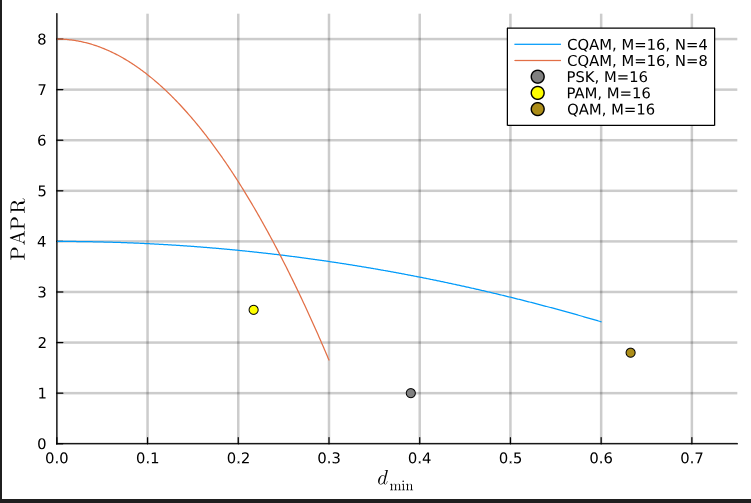
\includegraphics[width=0.7\textwidth]{plot_fig1.png}
    \caption{PAPR versus $d_{\text{min}}$ of CQAM and some other modulation schemes.}
    \label{fig:papr_vs_dmin}
\end{figure}

\end{document}

